\section{Convex functions}
\subsection{Extended-valued functions}
\begin{definition}[Extended-valued function]
    A function $f: \R^n \longrightarrow \R$ is \emph{extended-valued} if its domain is $\R^n$ and its range is $\bar{\R} := \R \cup \{+\infty\}$.
\end{definition}

\begin{example}[Indicator function]
    We consider the indicator function of interval $[a, b]$:
    \begin{equation*}
        \ind_{[a,b]}(x) := \begin{cases*}
            0 & if $x\in[a,b]$ \\
            +\infty & otherwise
        \end{cases*}
    \end{equation*}
    \begin{figure}[H]
        \centering
        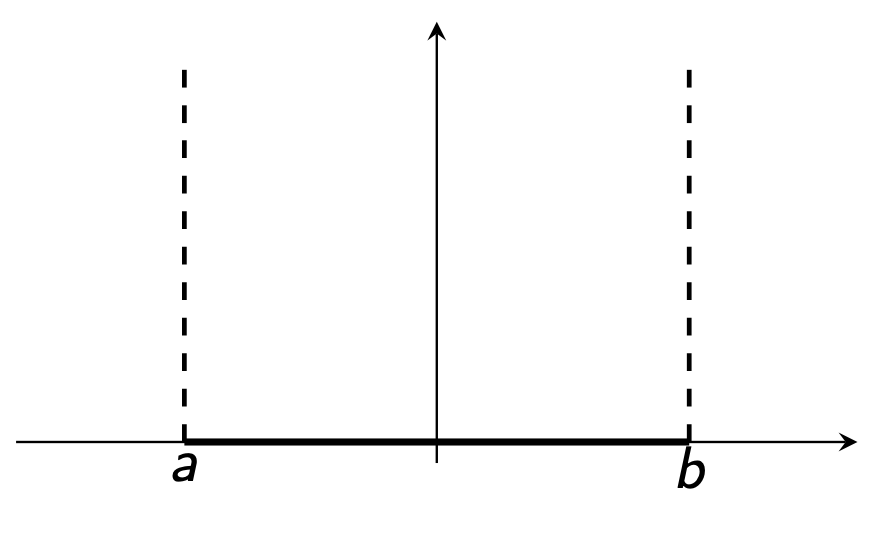
\includegraphics[width=.4\textwidth]{convex-functions/indicator.png}
    \end{figure}
\end{example}

\begin{definition}[Effective domain]
    The \emph{effective domain} of $f:\R^n\longrightarrow\bar{\R}$ is the set of points where $f$ is finite:
    \begin{equation}
        \dom f := \set{x\in\R^n}{f(x)<+\infty}
    \end{equation}
\end{definition}

A function is said to be \emph{proper} if its effective domain is non-empty: $\dom f \neq \emptyset$.

\subsection{Definition and first properties}
\begin{definition}[Convex function]
    A function $f:\R^n\longrightarrow\bar{\R}$ is \emph{convex} if its graph is below any line connecting two points of the graph $(x, f(x))$ and $(y, f(y))$. That is:
    \begin{equation}
        \forall x,y\in\R^n, \forall\theta\in[0,1], \quad f(\theta\cdot x + (1-\theta)\cdot y) \leq \theta\cdot f(x) + (1-\theta)\cdot f(y)
    \end{equation}
\end{definition}

\begin{definition}[Concave function]
    A function $f:\R^n\longrightarrow\bar{\R}$ is \emph{concave} if $-f$ is convex. That is:
    \begin{equation*}
        \forall x,y\in\R^n, \forall\theta\in[0,1], \quad f(\theta\cdot x + (1-\theta)\cdot y) \geq \theta\cdot f(x) + (1-\theta)\cdot f(y)
    \end{equation*}
\end{definition}

\begin{definition}[Epigraph]
    The \emph{epigraph} of a function $f:\R^n\longrightarrow\bar{\R}$ is the set of points lying above the graph of $f$:
    \begin{equation}
        \epi f := \set{(x, t)\in\R^n\times\R}{f(x)\leq t}
    \end{equation}
\end{definition}

\begin{property}[Convexity and epigraph]
    A function $f:\R^n\longrightarrow\bar{\R}$ is convex if and only if its epigraph is a convex set.

    \begin{figure}[H]
        \centering
        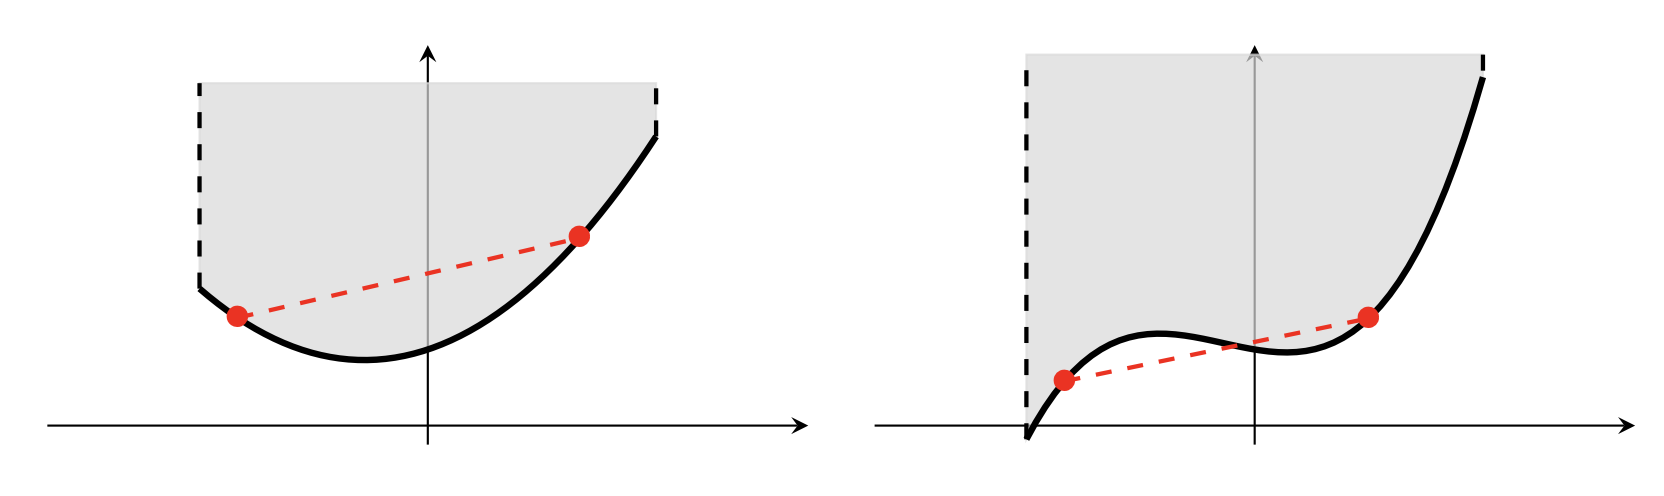
\includegraphics[width=.7\textwidth]{convex-functions/epigraph.png}
    \end{figure}
\end{property}

The following property allows to check the convexity of a multivariate function $f$ by checking the convexity of functions of one variable.
\begin{property}
    \label{prop:convexity-1d}
    Let $f:\R^n\longrightarrow\bar{\R}$ be a function, and let $x\in\dom f$. We define:
    \begin{equation*}
        \begin{aligned}
            g_{x,v} : \R &\longrightarrow \bar{\R} \\
            t &\longmapsto f(x+tv)
        \end{aligned}
    \end{equation*}
    with $\dom g_{x,v} = \set{t\in\R}{x+tv\in\dom f}$. Then, $f$ is convex if and only if $g_{x,v}$ is convex in $t$ for all $x\in\dom f$ and all $v\in\R^n$.
\end{property}

\begin{definition}[Sublevel sets]
    Let $f:\R^n\longrightarrow\bar{\R}$ be a function. The \emph{sublevel set} of $f$ at level $\alpha\in\R$ is the set of points lying below the level $\alpha$:
    \begin{equation*}
        S_\alpha(f) = \set{x\in\R^n}{f(x)\leq\alpha}
    \end{equation*}
\end{definition}

\begin{property}
    If $f$ is convex, then its sublevel sets are convex:
    \begin{equation*}
        f \text{ is convex} \implies \forall \alpha\in\R, \quad S_\alpha(f) \text{ is convex}
    \end{equation*}
    The converse is not true.
\end{property}

\subsection{First-order conditions}
\begin{property}[First-order condition for convexity]
    Let $f:\R^n\longrightarrow\bar{\R}$ be a differentiable function, that is that $\nabla f(x)$ exists for all $x\in\dom f$. Then, $f$ is convex if and only if $\dom f$ is convex and:
    \begin{equation*}
        \forall x,y\in\dom f, \quad f(y) \geq f(x) + \nabla f(x)^\top(y-x)
    \end{equation*}
\end{property}

In general, the function $f$ might not be differentiable. In this case, we can use the subdifferential, a generalization of the local variation of a function, to characterize the convexity of $f$.

Recall that a supporting hyperplane $(g, -1)$ of $\epi f$ at $(x, f(x))$ is a hyperplane such that:
\begin{equation*}
    \forall y\in\R^n, \quad f(y) \geq f(x) + g^\tp(y-x)
\end{equation*}
This motivates the following definition.

\begin{figure}[H]
    \centering
    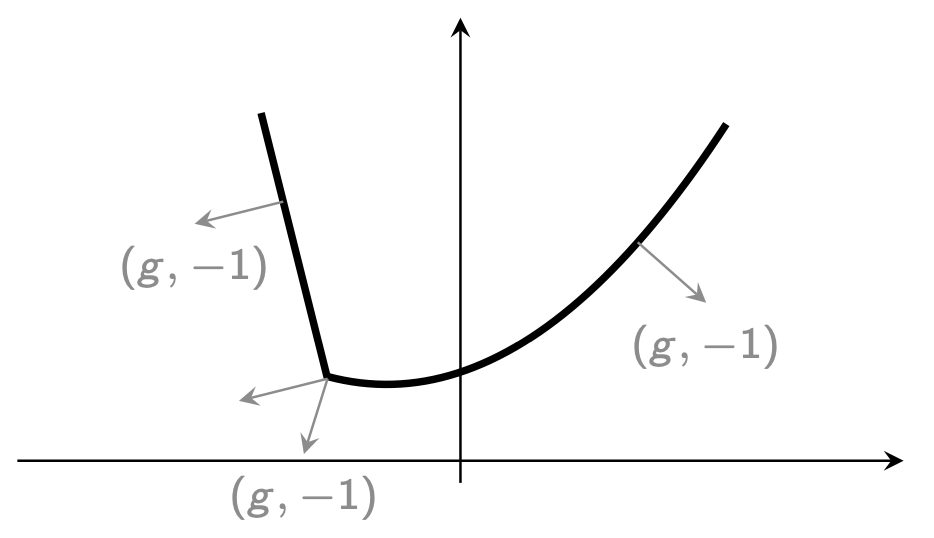
\includegraphics[width=.5\textwidth]{convex-functions/subdifferential.png}
\end{figure}

\begin{definition}[Subdifferential]
    The \emph{subdifferential} of a function $f:\R^n\longrightarrow\bar{\R}$ is the function associating to each point $x$ the set of all supporting hyperplanes of $\epi f$ at $(x, f(x))$:
    \begin{equation*}
        \begin{aligned}
            \partial f(x) : \R^n &\longrightarrow \Pc(\R^n) \\
            x &\longmapsto \set{g\in\R^n}{\forall y\in\R^n, \quad f(y) \geq f(x) + g^\tp(y-x)}
        \end{aligned}
    \end{equation*}
    Any $g\in\partial f(x)$ is called a \emph{subgradient} of $f$ at $x$.
\end{definition}

\begin{itemize}
    \item If $f$ is differentiable at $x$ and $\partial f(x)\neq\emptyset$, then $\partial f(x) = \{\nabla f(x)\}$.
    \item If $f$ is convex, and $\partial f(x)$ is a singleton, then $\partial f(x) = \{\nabla f(x)\}$.
    \item If $f$ is convex but not differentiable at $x\in\interior\dom f$, then:
    \begin{equation}
        \partial f(x) = \overline{\Conv S(x)}
    \end{equation}
    where $S(x) = \set{s\in\R^n}{\nabla f(x_k) \xrightarrow[x_k\to x]{} s}$
    \item In general, for a convex function $f$:
    \begin{equation}
        \partial f(x) = \overline{\Conv S(x)} + N_{\dom f}(x)
    \end{equation}
\end{itemize}

\begin{property}[Existence of subgradient]
    For finite-valued convex functions, a subgradient exists for every $x$.
\end{property}

\begin{property}[Existence of subgradient for extended-valued functions]
    In the extendevalued setting, let $f:\R^n\longrightarrow\bar{\R}$ be a convex function. Then:
\begin{enumerate}
    \item Subgradients exist for all $x$ in the relative interior of $\dom f$.
    \item Subgradients sometimes exist for $x$ on the relative boundary of $\dom f$.
    \item No subgradient exists for $x$ ourside of $\dom f$.
\end{enumerate}

\end{property}
\begin{figure}[H]
    \centering
    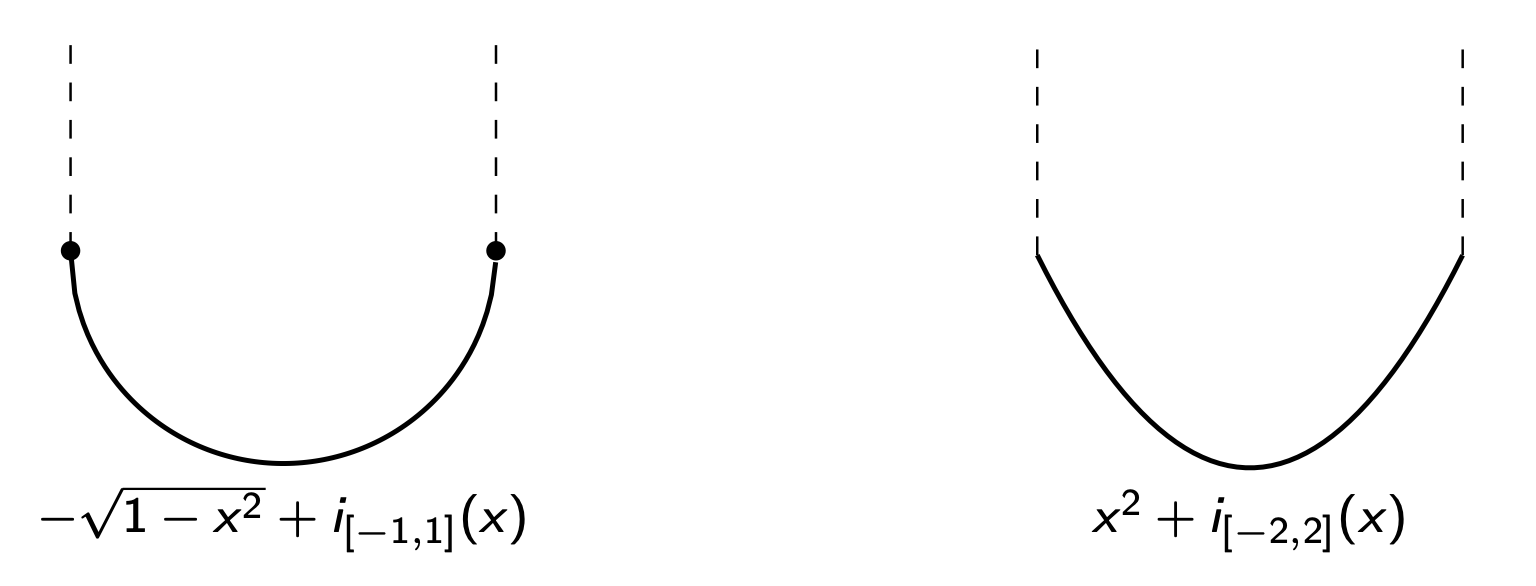
\includegraphics[width=.55\textwidth]{convex-functions/boundary.png}
    \caption{Examples for the second case, where boundary points exist on the relative boundary of $\dom f$. No subgradient (affine minorizer) exists for the left function at $x=\pm1$.}
\end{figure}

\subsection{Second-order conditions}
\begin{property}[Second-order condition for convexity]
    Let $f:\R^n\longrightarrow\bar{\R}$ be a twice differentiable function (i.e.~$\nabla^2f(x)$ exists for all $x\in\dom f$ which is open). Then, $f$ is convex if and only if $\dom f$ is convex and:
    \begin{equation}
        \forall x\in\dom f,\quad \nabla^2 f(x) \succcurlyeq 0
    \end{equation}
\end{property}

\subsection{Examples}
In practice, we showed multiple practical ways to establish the convexity of a function:
\begin{itemize}
    \item By definition, using the convexity criterion.
    \item By the existence of subgradients for all points of the domain.
    \item For twice differentiable functions, by checking the positive semidefiniteness of the Hessian.
    \item By decomposing the function into simpler functions through operations that preserve convexity.
\end{itemize}

\subsubsection{One-dimensional examples}
The following functions are convex:
\begin{itemize}
    \item affine functions: $x\longmapsto ax+b$, $a,b\in\R$
    \item exponential functions: $x\longmapsto e^{ax}$, $a\in\R$
    \item power functions: $x:\R^*_+ \longmapsto x^\alpha$, $a\geq 1$ or $\alpha\leq0$
    \item powers of absolute value: $x\longmapsto |x|^p$, $p\geq 1$
    \item negative entropy: $x:\R^*_+ \longmapsto x\log x$
\end{itemize}

The following functions are concave:
\begin{itemize}
    \item affine functions: $x:\longmapsto ax+b$, $a,b\in\R$ (both convex and concave)
    \item power functions: $x:\R^*_+ \longmapsto x^\alpha$, for $0\leq\alpha\leq1$
    \item logarithm: $x:\R^*_+ \longmapsto \log x$
\end{itemize}

\subsubsection{Examples on vectors}
The following functions are convex on $\R^n$:
\begin{itemize}
    \item affine functions $x\longmapsto a^\tp x + b$, $a\in\R^n$, $b\in\R$
    \item norms: $x\longmapsto \norm{x}_p = (\sum_{i=1}^n|x_i|^p)^{1/p}$, $p\geq 1$
    \item quadratic functions:
    \begin{equation*}
        f: x\longmapsto \frac{1}{2}x^\tp Px + q^\tp x + r
    \end{equation*}
    with $P\in\Sb^n$, $q\in\R^n$, $r\in\R$. Indeed, we have;
    \begin{equation*}
        \nabla f(x) = Px+q \quad \text{and} \quad \nabla^2 f(x) = P\succcurlyeq 0
    \end{equation*}
    \item least-squares objective:
    \begin{equation*}
        f: x\longmapsto \norm{Ax-b}_2^2
    \end{equation*}
    with $A\in\mathcal{M}_{m,n}(\R)$, $b\in\R^m$. Indeed, we have:
    \begin{equation*}
        \nabla f(x) = 2A^\tp(Ax-b) \quad \text{and} \quad \nabla^2 f(x) = 2A^\tp A\succcurlyeq 0
    \end{equation*}
\end{itemize}

\subsubsection{Examples on matrices}
The following functions are convex on $\mathcal{M}_{m,n}(\R)$:
\begin{itemize}
    \item affine functions (convex and concave):
    \begin{equation*}
        X \longmapsto \Tr(A^\tp X) + b = \sum_{i=1}^m\sum_{j=1}^n A_{i,j}X_{i,j} + b
    \end{equation*}
    \item spectral norm (maximum singular value):
    \begin{equation*}
        X \longmapsto \norm{X}_2 = \sigma_{\max}(X) = \sqrt{\lambda_{\max}(X^\tp X)}
    \end{equation*}
    \item in general, all norms are convex
\end{itemize}

\subsubsection{Log-determinant function}
The $\log\det$ function, defined on $\Sb^n$, is concave:
\begin{equation*}
    \begin{aligned}
        f: \Sb^n&\longrightarrow\R
        X &\longmapsto \log\det X
    \end{aligned}
\end{equation*}
with $\dom f = \Sb_{++}^n$. To show this, we will use Property \ref{prop:convexity-1d}; we define:
\begin{equation*}
    \begin{aligned}
        g_{X,V}: \R&\longrightarrow\R \\
        t &\longmapsto \log\det(X+tV)
    \end{aligned}
\end{equation*}
Note that:
\begin{equation*}
    \begin{aligned}
        g_{X,V}(t) 
        &= \log\det(X+tV) \\
        &= \log\det X + \log\det(I+tX^{-1/2}VX^{-1/2}) \\
        &= \log\det X + \sum_{i=1}^n \log(1+t\lambda_i)
    \end{aligned}
\end{equation*}
where $\lambda_i$ are the eigenvalues of $X^{-1/2}VX^{-1/2}$.

We then apply the second-order condition to $g_{X,V}$:
\begin{equation*}
    g_{X,V}''(t) = -\sum_{i=1}^n \frac{\lambda_i}{(1+t\lambda_i)^2} \leq 0
\end{equation*}
Therefore, $g_{X,V}$ is concave for any $X, V$, hence $f$ is concave.

\subsubsection{Softmax function}
The softmax function, defined on $\R^n$, is convex:
\begin{equation*}
    \begin{aligned}
        f: \R^n&\longrightarrow\R \\
        x &\longmapsto \log\sum_{i=1}^n e^{x_i}
    \end{aligned}
\end{equation*}
If we denote by $z_i = e^{x_i}/\sum_j e^{x_j}$, then we get:
\begin{equation*}
    \nabla^2 f(x) = \diag(z) - zz^\tp
\end{equation*}
with $z_i\geq0$ and $\sum_i z_i = 1$. To show that $\nabla^2 f(x)\succcurlyeq 0$, we show that $\diag(z) - zz^\tp$ is positive semidefinite. Let $v\in\R^n$, then:
\begin{equation*}
    \begin{aligned}
        v^\tp\nabla^2 f(x)v 
        &= v^\tp(\diag(z) - zz^\tp)v \\
        &= \sum_{i=1}^n z_i v_i^2 - \left(\sum_{i=1}^n z_i v_i\right)^2 \\
    \end{aligned}
\end{equation*}
According to the Cauchy-Schwarz inequality applied to $\sqrt{z_i}\times\sqrt{z_i}v_i$, we have:
\begin{equation*}
    \left(\sum_{i=1}^n z_i v_i\right)^2 \leq \sum_{i=1}^n z_i \sum_{i=1}^n z_i v_i^2 = \sum_{i=1}^n z_i v_i^2
\end{equation*}
Therefore, $v^\tp\nabla^2 f(x)v \geq 0$, and $f$ is convex.

\subsection{Convexity-preserving operations}
\subsubsection{Nonnegative weighted sum}
\begin{property}[Nonnegative scaling]
    Let $f:\R^n\longrightarrow\bar{\R}$ be a convex function, and $\alpha>0$. Then, $\alpha f$ is convex.
\end{property}

\begin{property}[Sum]
    Let $f_1, f_2:\R^n\longrightarrow\bar{\R}$ be convex functions. Then, $f_1+f_2$ is convex; this extends to infinite sums and integrals.
\end{property}

\begin{property}[Nonnegative weighted sum]
    Let $f_1, f_2:\R^n\longrightarrow\bar{\R}$ be convex functions, and $\alpha_1,\alpha_2>0$. Then, $\alpha_1f_1+\alpha_2f_2$ is convex; this extends to infinite sums and integrals.
\end{property}

\subsubsection{Compositions by an affine function}
\begin{property}[Composition by an affine function]
    Let $f:\R^n\longrightarrow\bar{R}$ be a convex function and let $A\in\mathcal{M}_{m,}(\R)$, $b\in\R^m$. Then:
    \begin{equation*}
        x\longmapsto f(Ax+b) \text{ is convex}
    \end{equation*}
\end{property}

\begin{example}
    The log barrier function for linear inequalities:
    \begin{equation*}
        f(x) = -\sum_{i=1}^m \log(b_i-a_i^\tp x)
    \end{equation*}
    with $\dom f=\set{x\in\R^n}{\forall i\in\iset{1}{m}, \quad a_i^\tp x<b_i}$, is convex.
\end{example}

\begin{example}
    Any norm of an affine function:
    \begin{equation*}
        f(x) = \norm{Ax+b}
    \end{equation*}
    is convex.
\end{example}

\subsubsection{Pointwise maximum}
\begin{property}[Pointwise maximum]
    Let $f_1, f_2:\R^n\longrightarrow\bar{\R}$ be convex functions. Then, $\max(f_1, f_2)$ is convex. This extends to the pointwise maximum of any finite number of convex functions.
\end{property}

\begin{example}
    The following piecewise linear function is convex:
    \begin{equation*}
        f(x) = \max_{i\in\iset{1}{m}} a_i^\tp x + b_i
    \end{equation*}

    \begin{figure}[H]
        \centering
        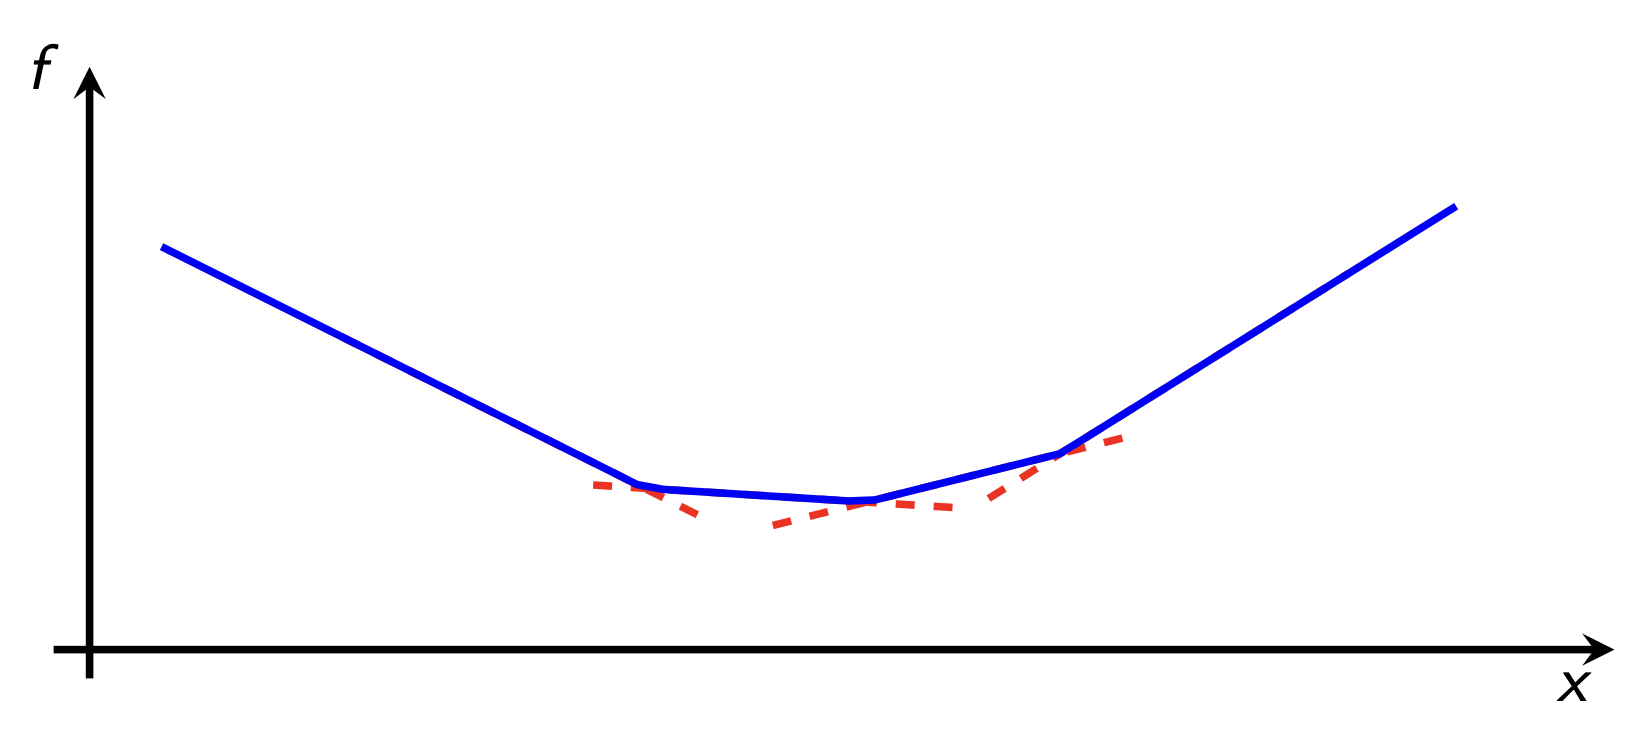
\includegraphics[width=.5\textwidth]{convex-functions/piecewise-linear.png}
    \end{figure}
\end{example}

\begin{example}[Sum of $r$ largest components]
    The sum of the $r$ largest components of a vector $x\in\R^n$ is convex:
    \begin{equation*}
        f(x) = x_{(1)} + \dots + x_{(r)}
    \end{equation*}
    where $x_{(1)}\geq\dots\geq x_{(n)}$ are the components of $x$ sorted in decreasing order.
    \begin{figure}[H]
        \centering
        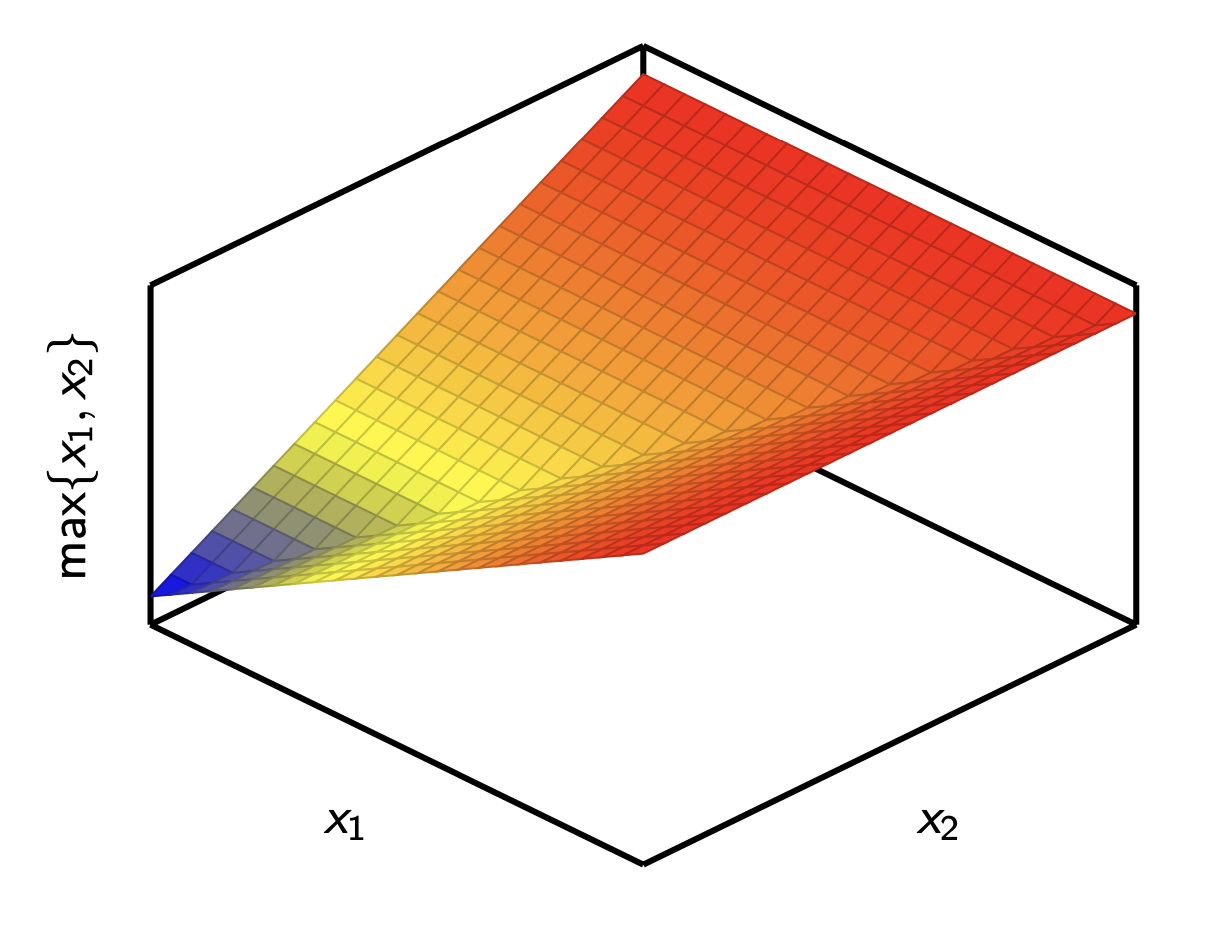
\includegraphics[width=.5\textwidth]{convex-functions/top-r.png}
    \end{figure}
    Indeed, we can write $f$ as:
    \begin{equation*}
        f(x) = \max\set{x_{i_1} + x_{i_2} + \dots + x_{i_r}}{1\leq i_1<i_2<\dots<i_r\leq n}
    \end{equation*}
\end{example}